\section{Reconstructing the exploration and pilot decisions}
\label{sec:results}

\subsection{Calibration coverage and reasons for rejection}

The reanalysis reconstructs seed contrasts for the privacy, utility and gain
exploration from archived losses, then checks the supplied cell and seed
tables. The pilot requires a separate calculation. We recompute paired
losses and candidate/null score arithmetic from 66 run-metrics records and
126 candidate score records, with the generated verification report as a
cross-check. These calculations use saved results throughout. Training,
probe fitting and scoring tensor captures lie outside this reanalysis.
Table~\ref{tab:cohorts} identifies the repetition units behind each summary.

\begin{table}[t]
\centering\small
\begin{tabularx}{\linewidth}{@{}lXX@{}}
\toprule
 & Exploration & Defence-redesign pilot \\
\midrule
Candidate configurations & \RoneCells & \PfourCells \\
Repetitions per candidate & 4 training seeds & 3 paired seeds \\
Recorded scope & Frozen exploratory rules & Frozen exploratory pilot \\
Qualified breach or failed composite & \RoneQualifiedBreaches & \PfourPrivacyFailures \\
Privacy undetermined & \RoneUndetermined & \PfourPrivacyUndetermined \\
Utility failures & \RoneUtilityFailures & \PfourUtilityFailures \\
Gain failures & \RoneGainFailures & 0 \\
Eligible candidate & None & None \\
\bottomrule
\end{tabularx}
\caption{\textbf{No candidate meets all three requirements.}
Exploration rejection reasons overlap. The pilot retains its recorded
composite privacy rule, so the two privacy rows represent different
estimands. Counts enumerate archived candidate configurations, with no
population frequency interval. The source records are \artifact{R1} and
\artifact{P4}.}
\label{tab:cohorts}
\end{table}

Thirteen exploration configurations have a qualified privacy breach.
The other six fail independent utility or gain criteria, so all 19 remain
rejected under the frozen finite protocol. Incomplete coverage cannot
explain these rejections away. Revising the instruments would need to
change the recorded rejection reasons before it could change that
conclusion.

The statistical conventions also differ between campaigns. The exploration
uses a two-sided 95\% seed interval, while the pilot uses a one-sided
95\% upper utility limit with $t_{0.95,2}=2.919986$ over three paired seeds.
We preserve each convention. Their distinction remains visible in the
checks and disjoint exploration reason intersections in
Appendix~\ref{app:checks}, rather than being absorbed into a common
confidence calculation.

The pilot also separates atomic measurements from the campaign's composite
privacy label. A qualified structure probe can detect a large signal even
when a missing property binding leaves the all-bindings assessment
undetermined. The atomic signal remains measurable. Retaining both results
preserves the source's aggregation policy and identifies the coverage
behind its verdict. Figure~\ref{fig:campaigns} presents the two campaigns
with their different metrics kept separate.

\begin{figure}[t]
\centering
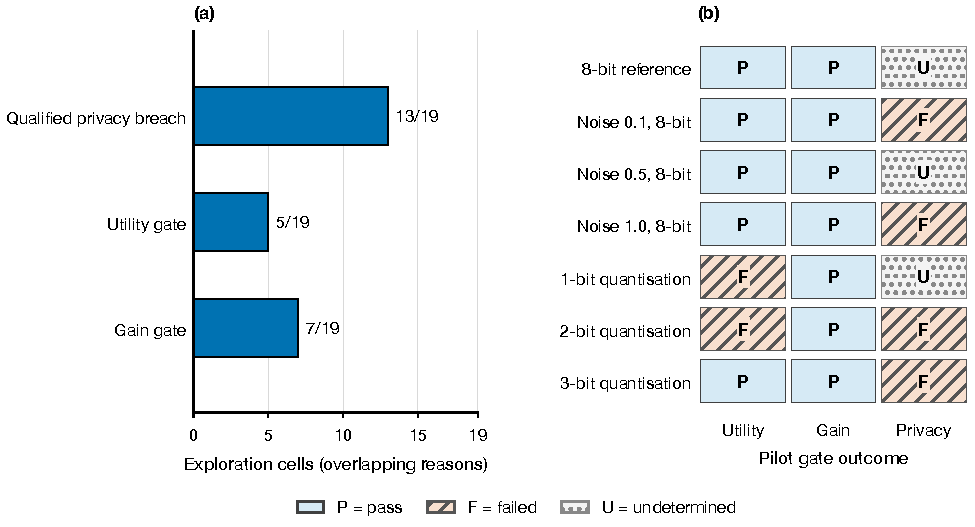
\includegraphics[width=\linewidth]{figs/campaign-gates.pdf}
\caption{\textbf{Qualified breaches remain valid despite incomplete coverage.}
The left panel shows overlapping rejection reasons among 19 exploration
configurations evaluated with four seeds each. The right panel gives the
recorded gate outcomes for seven pilot cells with three paired seeds.
The counts describe complete campaigns and carry no population sampling
interval. The source records are
\artifact{R1} and \artifact{P4}.}
\label{fig:campaigns}
\end{figure}

\subsection{The narrow utility margin still passes}

The exploration utility rule requires a mean difference between candidate
and baseline of at most $0.10$ nats and an upper 95\% Student-$t$ limit
of at most $0.12$ nats. Four seeds give the descriptive interval
\begin{equation}
 \bar u\;\pm\;t_{0.975,3}\,\frac{s_u}{\sqrt{4}},
 \qquad t_{0.975,3}\approx3.182446.
 \label{eq:interval}
\end{equation}
The fixed evaluation data define its scope. These intervals are
unadjusted across configurations and provide no independent corpus
replication. Figure~\ref{fig:utility} separates the two thresholds.

The span-6 configuration has mean $0.0999705344$ and upper limit
$0.1195024415$. Both recorded utility criteria are satisfied. Its mean
passes by $2.9466\times10^{-5}$ nats and its upper limit by
$4.9756\times10^{-4}$ nats. The saved rejection instead combines gain
failure with a qualified privacy breach. Depth-4 has a lower point estimate
than the base configuration. This comparison and its limited seed count
cannot establish a general depth law (\artifact{R1}).

\begin{figure}[t]
\centering
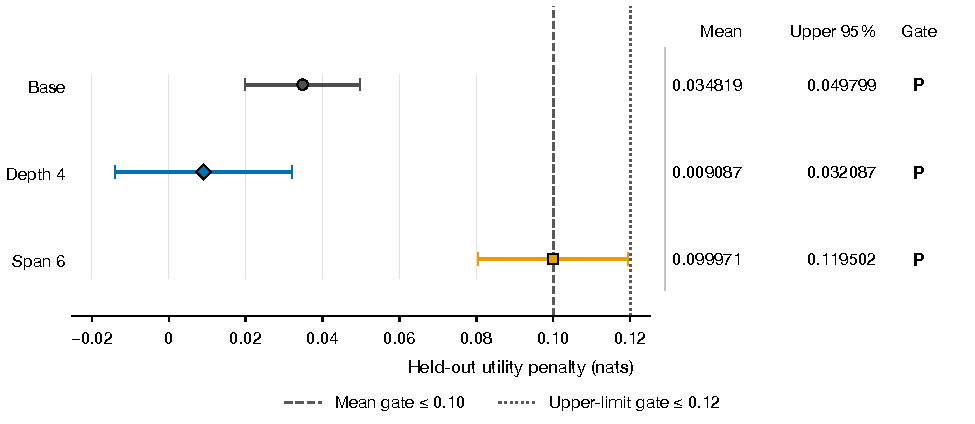
\includegraphics[width=\linewidth]{figs/r1-utility-boundary.pdf}
\caption{\textbf{Span-6 passes both recorded utility criteria.}
Means and descriptive two-sided 95\% Student-$t$ intervals across four
training seeds are conditional on fixed evaluation text. The $0.10$ mean
threshold and $0.12$ upper-limit threshold concern different statistics.
An interval endpoint can cross the mean threshold while the utility
criteria still pass. The source is \artifact{R1}. Intervals follow
Eq.~\eqref{eq:interval}.}
\label{fig:utility}
\end{figure}
\FloatBarrier
